\section{Results I: the transferred local correction (Amendment 1)}
\label{sec:results}

\subsection{All arms on the official folds}
Table~\ref{tab:arms} lists every arm on every task (mean $\pm$ standard deviation over the five official folds), and Table~\ref{tab:tests} the pre-registered tests.
The equal-weight mean of the experts is clearly the worst ensemble on all tasks; the simplex stack never loses to it.
Against the best single expert chosen by inner cross-validation, the stack is better on glass (\GlassStackVsBestSingleRel\% ROC-AUC, $p_\mathrm{boot}=\GlassStackVsBestSingleP$, 5/5 folds) and is within noise on the other three tasks (steels \SteelsStackVsBestSingleRel\%, expt\_gap \GapStackVsBestSingleRel\%, expt\_is\_metal \MetalStackVsBestSingleRel\%).
The extremely randomised trees expert carries most of the stack weight on the two regression tasks, and LightGBM and extra trees share it on the classification tasks (Table~\ref{tab:weights}).

\begin{table}[t]
\centering
\caption{Every arm on the four Matbench composition tasks (official 5-fold CV; mean $\pm$ s.d.\ over folds). Regression: MAE (lower is better); classification: ROC-AUC from probabilities (higher is better). Single-expert rows are means over the folds in which the expert was part of the selected configuration.}
\label{tab:arms}
\begin{adjustbox}{max width=\textwidth}
\begin{tabular}{lcccc}
\toprule
Arm & steels & expt\_gap & expt\_is\_metal & glass \\
 & MAE (MPa) & MAE (eV) & ROC-AUC & ROC-AUC \\
\midrule
Best single (inner CV) & 83.41 $\pm$ 10.86 & 0.3259 $\pm$ 0.0130 & 0.9819 $\pm$ 0.0015 & 0.9548 $\pm$ 0.0097 \\
Equal-weight mean & 102.46 $\pm$ 20.11 & 0.4007 $\pm$ 0.0242 & 0.9811 $\pm$ 0.0027 & 0.9458 $\pm$ 0.0116 \\
Simplex stack & 83.12 $\pm$ 10.89 & 0.3264 $\pm$ 0.0139 & 0.9825 $\pm$ 0.0017 & 0.9567 $\pm$ 0.0091 \\
Stack + local corr. (naive) & 82.80 $\pm$ 11.65 & 0.3240 $\pm$ 0.0140 & 0.9825 $\pm$ 0.0018 & 0.9567 $\pm$ 0.0091 \\
\quad ablation: Magpie space only & 83.53 $\pm$ 11.30 & 0.3235 $\pm$ 0.0139 & 0.9825 $\pm$ 0.0017 & 0.9567 $\pm$ 0.0091 \\
\quad ablation: fraction space only & 82.80 $\pm$ 11.65 & 0.3235 $\pm$ 0.0142 & 0.9825 $\pm$ 0.0018 & 0.9567 $\pm$ 0.0091 \\
Stack + fold-matched corr. & 82.02 $\pm$ 9.12 & 0.3276 $\pm$ 0.0149 & 0.9826 $\pm$ 0.0017 & 0.9559 $\pm$ 0.0094 \\
Best single + local corr. & 82.69 $\pm$ 11.60 & 0.3239 $\pm$ 0.0133 & 0.9819 $\pm$ 0.0015 & 0.9548 $\pm$ 0.0097 \\
\midrule
Expert et\_all & 83.41 & 0.3259 & 0.9809 & 0.9548 \\
Expert krr\_frac & 160.38 & 0.5613 & -- & -- \\
Expert krr\_magpie & 109.37 & 0.4840 & -- & -- \\
Expert lgbm\_all & 88.00 & 0.3425 & 0.9819 & 0.9519 \\
Expert lgbm\_l1\_all & 93.97 & -- & -- & -- \\
Expert mlp\_all & 156.17 & 0.4611 & 0.9702 & 0.9055 \\
Expert rf\_all & 96.62 & 0.3645 & 0.9808 & 0.9516 \\
Expert svc\_frac & -- & -- & 0.9472 & 0.8735 \\
Expert svc\_magpie & -- & -- & 0.9566 & 0.9009 \\
\bottomrule
\end{tabular}

\end{adjustbox}
\end{table}

\begin{table}[t]
\centering
\caption{Pre-registered primary test (naive local correction vs.\ uncorrected stack) and key secondary comparisons. $\Delta$ is the mean over folds of the metric difference (MAE for regression, where negative favours A; ROC-AUC for classification, where positive favours A). CI and $p_\mathrm{boot}$: paired bootstrap over test points within folds ($B=10^4$); $p_\mathrm{Holm}$: Holm correction over the four primary tests; $p_\mathrm{NB}$: Nadeau--Bengio corrected resampled $t$-test over the five folds.}
\label{tab:tests}
\begin{adjustbox}{max width=\textwidth}
\begin{tabular}{llcccccc}
\toprule
Task & Comparison (A vs B) & $\Delta$ = A$-$B (rel.) & 95\% CI & $p_\mathrm{boot}$ & $p_\mathrm{Holm}$ & folds A better & $p_\mathrm{NB}$ \\
\midrule
steels & naive local vs stack (primary) & -0.3202 (-0.39\%) & [-2.15, +1.5] & 0.720 & 1.000 & 3/5 & 0.896 \\
steels & naive local vs best single & -0.6135 (-0.74\%) & [-2.63, +1.34] & 0.538 & -- & 3/5 & 0.816 \\
steels & stack vs best single & -0.2933 (-0.35\%) & [-1.65, +1.08] & 0.660 & -- & 2/5 & 0.417 \\
steels & fold-matched vs stack & -1.097 (-1.32\%) & [-4.32, +2.13] & 0.519 & -- & 2/5 & 0.817 \\
steels & fold-matched vs naive local & -0.7765 (-0.94\%) & [-3.45, +1.91] & 0.583 & -- & 3/5 & 0.812 \\
\addlinespace
expt\_gap & naive local vs stack (primary) & -0.00232 (-0.71\%) & [-0.0037, -0.000942] & 0.001 & 0.005 & 5/5 & 0.011 \\
expt\_gap & naive local vs best single & -0.001895 (-0.58\%) & [-0.00391, +0.000155] & 0.071 & -- & 4/5 & 0.108 \\
expt\_gap & stack vs best single & +0.0004248 (+0.13\%) & [-0.000988, +0.00181] & 0.566 & -- & 3/5 & 0.695 \\
expt\_gap & fold-matched vs stack & +0.001241 (+0.38\%) & [-0.00145, +0.00418] & 0.390 & -- & 2/5 & 0.516 \\
expt\_gap & fold-matched vs naive local & +0.00356 (+1.10\%) & [+0.0012, +0.00602] & 0.005 & -- & 0/5 & 0.096 \\
\addlinespace
expt\_is\_metal & naive local vs stack (primary) & -3.305e-06 (-0.00\%) & [-4.88e-05, +4.3e-05] & 0.899 & 1.000 & 0/5 & 0.541 \\
expt\_is\_metal & naive local vs best single & +0.0005853 (+0.06\%) & [-0.000504, +0.0017] & 0.301 & -- & 4/5 & 0.348 \\
expt\_is\_metal & stack vs best single & +0.0005886 (+0.06\%) & [-0.000507, +0.0017] & 0.275 & -- & 4/5 & 0.345 \\
expt\_is\_metal & fold-matched vs stack & +0.0001571 (+0.02\%) & [-0.000148, +0.00047] & 0.320 & -- & 3/5 & 0.577 \\
expt\_is\_metal & fold-matched vs naive local & +0.0001604 (+0.02\%) & [-0.000128, +0.000458] & 0.277 & -- & 3/5 & 0.566 \\
\addlinespace
glass & naive local vs stack (primary) & +0 (+0.00\%) & [+0, +0] & 1.000 & 1.000 & 0/5 & 1.000 \\
glass & naive local vs best single & +0.001897 (+0.20\%) & [+0.000704, +0.00314] & 0.002 & -- & 5/5 & 0.141 \\
glass & stack vs best single & +0.001897 (+0.20\%) & [+0.000689, +0.00314] & 0.002 & -- & 5/5 & 0.141 \\
glass & fold-matched vs stack & -0.0008173 (-0.09\%) & [-0.00194, +0.000315] & 0.153 & -- & 1/5 & 0.247 \\
glass & fold-matched vs naive local & -0.0008173 (-0.09\%) & [-0.00192, +0.000273] & 0.149 & -- & 1/5 & 0.247 \\
\bottomrule
\end{tabular}

\end{adjustbox}
\end{table}

\subsection{Primary endpoint: does the local correction transfer?}
The correction improved \NTasksImproved{} of the four tasks under the pre-registered rule.
On expt\_gap the corrected stack reached an MAE of \GapStackLocal{}~eV against \GapStack{}~eV for the uncorrected stack ($\Delta=\DeltaGap$~eV, \RelGap\%), with every one of the five folds improved and $p_\mathrm{Holm}=\PHolmGap$ (Nadeau--Bengio $p=\PNBGap$).
The effect is real but small: about 0.7\% of the MAE.
On steels the change was \RelSteels\% ($p_\mathrm{Holm}=\PHolmSteels$, \FoldsSteels{}/5 folds improved), indistinguishable from zero given a fold-to-fold standard deviation of about \SteelsStackStd~MPa.
On the two classification tasks the inner-CV selection almost never switched the correction on (glass: \GlassNaiveOn/5 folds; expt\_is\_metal: \MetalNaiveOn/5), so the corrected and uncorrected stacks are identical or nearly so ($\Delta$ ROC-AUC $=\DeltaMetal$ and $\DeltaGlass$).
In short, the correction that was confirmed in our chemistry study transfers only weakly: it gives a consistent sub-percent gain on the largest regression task, nothing measurable on steels, and is (correctly) declined by its own selection procedure on the classification tasks.

\subsection{Where the correction helps and hurts}
Fig.~\ref{fig:support} stratifies the test errors by the distance from each test composition to its nearest training composition.
On both regression tasks the naive correction \emph{hurt} in the nearest-support quartile (expt\_gap \GapLocalQOne\%, steels \SteelsLocalQOne\% MAE relative to the stack) and helped in the other three (expt\_gap \GapLocalQTwo\%, \GapLocalQThree\%, \GapLocalQFour\%).
That is the pattern the fold-matched analysis predicts: for a near-duplicate neighbour the deployed stack has already absorbed the neighbour's error, so adding its OOF residual counts it twice.
The fold-matched variant, however, did not repair it: on expt\_gap it was worse than the naive correction overall (\GapStackFmVsStackLocalRel\% MAE, $p_\mathrm{boot}=\GapStackFmVsStackLocalP$, 0/5 folds better) and also worse in the nearest quartile (\GapFmQOne\%).
On steels it gave the lowest mean MAE of all arms (\SteelsStackFm~MPa) but with no detectable difference from the stack (\SteelsStackFmVsStackRel\%, $p_\mathrm{boot}=\SteelsStackFmVsStackP$).
On the classification tasks it was switched on in every fold but changed ROC-AUC by less than 0.1\% in either direction.

\begin{figure}[t]
\centering
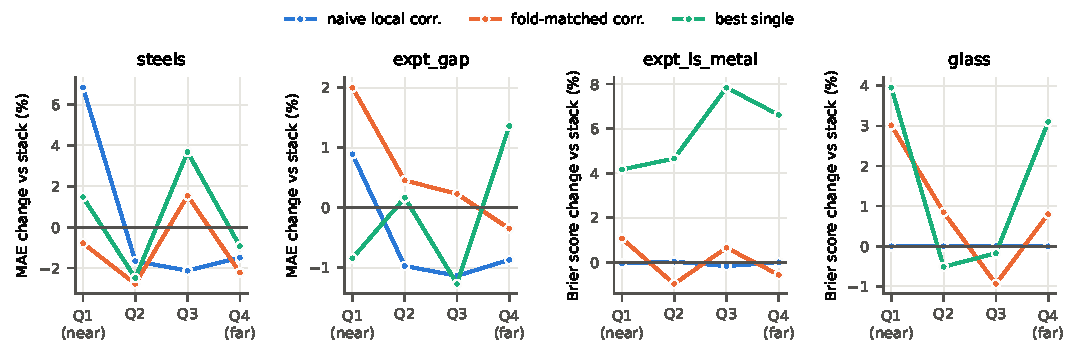
\includegraphics[width=\textwidth]{figures/fig_support.pdf}
\caption{Error change relative to the uncorrected stack, by support quartile (distance from the test composition to its nearest training composition; bin edges are the training rows' leave-one-out quartiles in each fold). Regression: MAE; classification: Brier score. Negative is better.}
\label{fig:support}
\end{figure}

\begin{figure}[t]
\centering
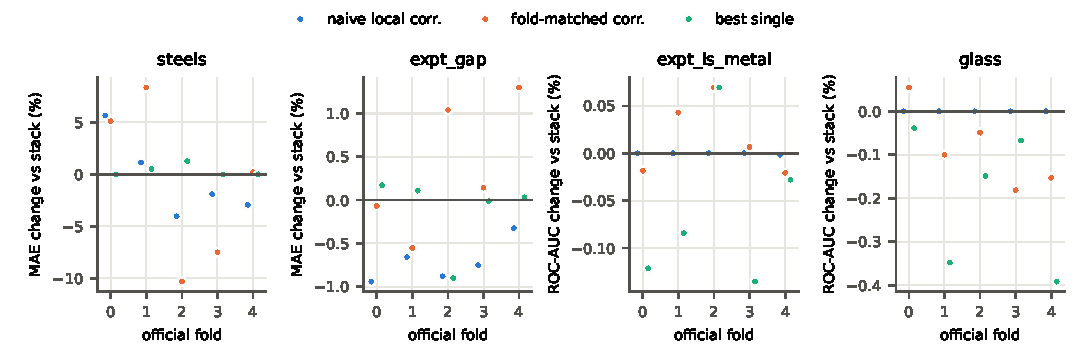
\includegraphics[width=\textwidth]{figures/fig_perfold.pdf}
\caption{Per-fold change of the test metric relative to the uncorrected stack for the naive and fold-matched corrections and the best single expert (selected by inner CV). For classification a positive change in ROC-AUC is better.}
\label{fig:perfold}
\end{figure}

\subsection{Ablations and controls}
Restricting the neighbour search to one composition space gave essentially the same gain on expt\_gap (Magpie \GapStackLocalMagpieVsStackRel\%, element fractions \GapStackLocalFracVsStackRel\%), whereas on steels only the element-fraction space was selected in practice and the Magpie-only variant was slightly worse than the stack (\SteelsStackLocalMagpieVsStackRel\%, 0/5 folds better).
Applying the correction to the best single expert instead of the stack (``correction without stacking'') improved expt\_gap by \GapSingleLocalVsBestSingleRel\% relative to that expert ($p_\mathrm{boot}=\GapSingleLocalVsBestSingleP$, 5/5 folds), so on this task the gain does not depend on stacking.
The label-permutation control did not behave as a clean null: with labels permuted within inner folds the selection still switched a correction on in every fold of every task (Table~\ref{tab:selections}), because shrinking predictions toward a neighbourhood mean lowers the training loss against permuted labels too.
We pre-registered this control as diagnostic only, and it shows that a non-zero selected strength is not by itself evidence of local structure.

\begin{table}[t]
\centering
\caption{Number of official folds (of 5) in which the inner-CV selection switched each correction on, and the same for the label-permutation control.}
\label{tab:selections}
\begin{adjustbox}{max width=\textwidth}
\begin{tabular}{lcccc}
\toprule
Task & naive corr. on & fold-matched corr. on & perm.\ control on (naive) & perm.\ control on (f.-m.) \\
\midrule
steels & 5/5 & 5/5 & 5/5 & 5/5 \\
expt\_gap & 5/5 & 5/5 & 5/5 & 5/5 \\
expt\_is\_metal & 1/5 & 5/5 & 5/5 & 5/5 \\
glass & 0/5 & 5/5 & 5/5 & 5/5 \\
\bottomrule
\end{tabular}

\end{adjustbox}
\end{table}

\subsection{Comparison with the Matbench leaderboard}
Table~\ref{tab:board} places the pre-registered primary arm on the leaderboard snapshot of 18 October 2026.
For the classification tasks we compare balanced accuracy at the inner-CV threshold with the board's balanced-accuracy column, because the board's ``ROC-AUC'' values of the label-based entries equal their balanced accuracy.
The method would rank \SteelsRank{} of \SteelsNEntries{} on steels (behind TPOT-Mat and AutoML-Mat, ahead of MODNet v0.1.12), \GapRank{} of \GapNEntries{} on expt\_gap (behind Darwin, ahead of the CrabNet and MODNet entries), \MetalRank{} of \MetalNEntries{} on expt\_is\_metal and \GlassRank{} of \GlassNEntries{} on glass.
It does not beat the best entry on any task.
On expt\_gap and glass the gaps to the leaders are large (\GapStackLocal{} vs.\ 0.2865~eV; balanced accuracy \GlassStackLocalBA{} vs.\ 0.9603), and on expt\_is\_metal it is 0.023 in balanced accuracy.
Our probability ROC-AUCs (\MetalAUCprob{} on expt\_is\_metal, \GlassAUCprob{} on glass) are not comparable with the label-based board values and are not ranked.

\begin{table}[t]
\centering
\caption{Primary arm versus the Matbench v0.1 leaderboard (snapshot 18 October 2026). Classification: balanced accuracy at the threshold chosen inside each training fold, compared with the board's balanced-accuracy column. Rank counts our entry among the board entries.}
\label{tab:board}
\begin{adjustbox}{max width=\textwidth}
\begin{tabular}{llccc}
\toprule
Task & Metric & Ours: stack + naive corr. & Best board entry & Rank \\
\midrule
steels & MAE & 82.80 $\pm$ 11.65 & TPOT-Mat: 79.95 $\pm$ 13.59 & 3 of 12 \\
expt\_gap & MAE & 0.3240 $\pm$ 0.0140 & Darwin: 0.2865 $\pm$ 0.0083 & 2 of 13 \\
expt\_is\_metal & balanced acc. & 0.9370 $\pm$ 0.0063 & Darwin: 0.9598 & 2 of 8 \\
glass & balanced acc. & 0.8841 $\pm$ 0.0184 & MODNet (v0.1.12): 0.9603 & 2 of 8 \\
\bottomrule
\end{tabular}

\end{adjustbox}
\end{table}

\subsection{Calibration and compute}
Stacking improved the Brier score and the expected calibration error over the best single expert on both classification tasks, and the corrections left them essentially unchanged (Table~\ref{tab:calib}).
On 24 CPU cores (5 parallel workers of 4 threads) one official fold took a median of about \SteelsScratchMin, \GapScratchMin, \MetalScratchMin{} and \GlassScratchMin{} minutes for steels, expt\_gap, expt\_is\_metal and glass when every expert was computed from scratch (the glass figure includes a system-standby pause); the pair-excluded refits of the fold-matched arm account for \SteelsPairShare\%, \GapPairShare\% and \MetalPairShare\% of the expert-fitting time on the first three tasks (\GlassPairShare\% on glass, inflated by the same pause).

\begin{table}[t]
\centering
\caption{Calibration on the classification tasks (means over folds) and balanced accuracy at the inner-CV threshold.}
\label{tab:calib}
\begin{adjustbox}{max width=\textwidth}
\begin{tabular}{llcccc}
\toprule
Task & Arm & Brier & log loss & ECE & bal.\ acc. \\
\midrule
expt\_is\_metal & Best single & 0.0498 & 0.2007 & 0.0369 & 0.9378 \\
expt\_is\_metal & Stack & 0.0469 & 0.1662 & 0.0201 & 0.9374 \\
expt\_is\_metal & Stack + naive corr. & 0.0468 & 0.1662 & 0.0192 & 0.9370 \\
expt\_is\_metal & Stack + fold-matched corr. & 0.0469 & 0.1660 & 0.0211 & 0.9366 \\
glass & Best single & 0.0747 & 0.2451 & 0.0220 & 0.8827 \\
glass & Stack & 0.0735 & 0.2398 & 0.0211 & 0.8841 \\
glass & Stack + naive corr. & 0.0735 & 0.2398 & 0.0211 & 0.8841 \\
glass & Stack + fold-matched corr. & 0.0740 & 0.2411 & 0.0232 & 0.8835 \\
\bottomrule
\end{tabular}

\end{adjustbox}
\end{table}

\begin{table}[t]
\centering
\caption{Mean simplex-stack weight per expert (over folds; ``--'' where the expert was not in the selected configuration of every fold).}
\label{tab:weights}
\begin{adjustbox}{max width=\textwidth}
\begin{tabular}{lcccc}
\toprule
Expert & steels & expt\_gap & expt\_is\_metal & glass \\
\midrule
et\_all & 0.94 & 0.86 & 0.41 & 0.57 \\
krr\_frac & 0.00 & 0.00 & -- & -- \\
krr\_magpie & 0.06 & 0.00 & -- & -- \\
lgbm\_all & 0.00 & 0.14 & 0.48 & 0.27 \\
lgbm\_l1\_all & -- & -- & -- & -- \\
mlp\_all & 0.00 & 0.00 & 0.05 & 0.00 \\
rf\_all & 0.00 & 0.00 & 0.03 & 0.10 \\
svc\_frac & -- & -- & 0.01 & 0.06 \\
svc\_magpie & -- & -- & 0.02 & 0.00 \\
\bottomrule
\end{tabular}

\end{adjustbox}
\end{table}
